\toclesssection{SCP 021 - Skin Wyrm}
\addcontentsline{toc}{section}{SCP 021 - Skin Wyrm}

\textbf{Item \#:} SCP-021

\textbf{Object Class:} Safe

\begin{figure}[h]
\begin{center}
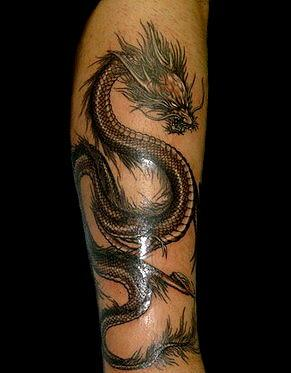
\includegraphics[scale=0.6]{scp/021.jpg}
\linebreak SCP-021 on subject D-124 (now deceased)
\end{center}
\end{figure}

\textbf{Special Containment Procedures:} SCP-021 is an obligate parasite of the human body. Containment, therefore, is no more difficult than containing an adult human; most cells will suffice. Item is currently housed in detention cell 217-A on subject D-139. Only class D personnel are eligible for hosting SCP-021. As long as a given subject survives as a host for SCP-021, he is exempt from normal monthly terminations of class D personnel.

\textbf{Description:} SCP-021 takes the form of a large and elaborate tattoo of a serpentine dragon in the oriental style, covering approximately 0.8 square meters of skin. This tattoo is fully animate within the confines of its host's skin and behaves largely as a normal animal would, albeit in only two dimensions. The tattoo's movement causes constant pain to its host, comparable and similar in character to simultaneous tattooing and tattoo removal on a large scale. The organism tends to spend most of its time on and near the torso. SCP-021 displays no intelligence beyond a basic pattern of feeding and locomotion, although actually measuring the intelligence of a two-dimensional life-form has proven impossible thus far.

SCP-021 appears to feed exclusively on pigments in the host's skin. This can include melanin, in which case the subject appears to be suffering from vitiligo. However, the organism shows a marked preference for other tattoos and will seek out and devour these before resorting to natural pigments. It should be noted that the feeding process itself, beyond the sensation of movement, is painless; normal tattoo ink simply vanishes as it is 'eaten'. The organism maintains a constant size, and no excretions have been observed. The organism is capable of clearing over 0.6 square meters of skin per hour. One may 'feed' SCP-021 by (quickly) tattooing fruits or small animals on the host.

SCP-021 can be transferred between hosts by various forms of physical contact, with differing rates of success. In the case of successful transfer, the organism simply 'swims' from one person to the other. Sexual intercourse appears to be the most reliable method of transfer, with a 93\% rate of transmission. However, due to the severe pain involved, this is less than ideal. Contact between two open wounds is generally preferable. Transfer is more complicated in deceased subjects, though not unreasonably so; the organism suffers no ill effects from the death of its host and continues to consume pigments. Transmission between species is unknown; previous tests suggest it to be either impossible or exceedingly rare.

SCP-021 does confer some benefits to its host. The tattoo has been proven to accelerate the release and re-uptake of epinephrine and decrease lactic acid buildup, providing boosts of strength, confidence, and pain tolerance in stressful situations and reducing the usual after-effects of weakness and fatigue. In addition, the tattoo seems to have some beneficial effect on the host's immune system. Aggression profiles in hosts are generally higher than average, though whether this is a direct effect of the tattoo or simply a reaction to the constant pain remains to be seen.
\newpage
The symbiotic relationship is usually limited by how long the host can tolerate such pain in everyday life. This has culminated in suicide in a number of subjects. In rare cases, hosts have also fallen victim to fatal skin infections.

SCP-021's origins and nature are a mystery. Tracing its transmission from host to host is hardly feasible within the confines of secrecy, and the organism could well be hundreds of years old, if not more. Nevertheless, SCP-021's captivity is one of the longest in the Foundation's history at nearly \expunged \ years, and has been very educational thus far. Current research focuses mainly on observing the characteristics of life in two dimensions.